\section{Einf�hrung in die Katalyse}
\subsection{Grundlagen}
Ein Katalysator
\begin{itemize}
\item beschleunigt eine chemische Reaktion, ohne das thermodynamische Gleichgewicht der Reaktion zu verschieben.
\item er�ffnet einen neuen Reaktionsweg mit geringerer Aktivierungsenergie.
\item vermeidet stabile Zwischenprodukte durch den katalytischen Reaktionsweg.
\end{itemize}
Vorteile sind demnach:
\begin{itemize}
\item milde Reaktionsbedingungen
\item Kosteneffizienz
\item Umweltfreundlichkeit
\end{itemize}
Die G�te eines Katalysators wird durch folgende Merkmale bestimmt:
\begin{enumerate}
\item Selektivit�t
\item Aktivit�t
\item Lebensdauer
\end{enumerate}
\begin{figure}[H]
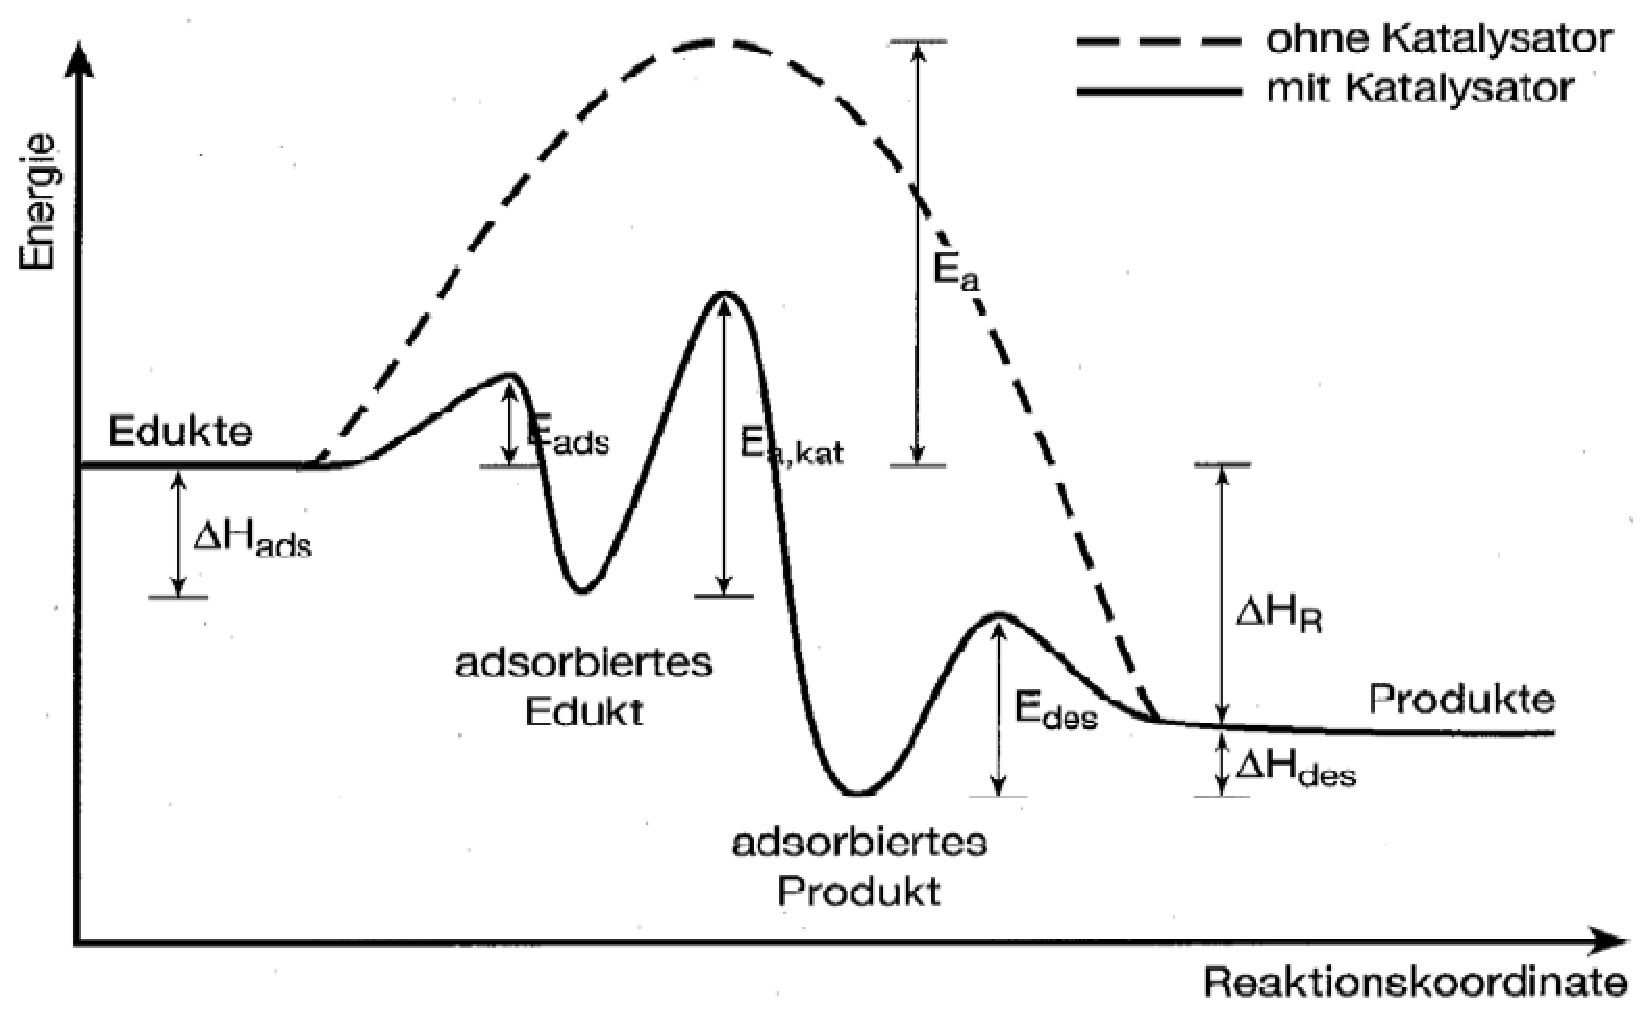
\includegraphics[width=87mm]{images/katalyse.eps}
\end{figure}

\subsection{Katalytischer Kreislauf}
\begin{enumerate}
\item Aktivierung des Katalysators
\item Aktiver Katalysator bindet an Substrat I
\item Der Katalysator-Substrat-Komplex bindet an Substrat II
\item Es bildet sich ein �bergangszustand, welcher in einen Katalysator-Produkt-Komplex �bergeht
\item Produkt und Katalysator trennen sich und es geht bei (2) weiter.
\end{enumerate}

\subsection{Homogene und Heterogene Katalyse}
\begin{table}[H]
\begin{tabular}{l|c|c}
		& \bf Homogen	& \bf Heterogen \\ \hline
Aktivit�t	& hoch		& variabel \\ 
Selektivit�t	& hoch		& variabel\\ 
Reakt.bed.	& mild		& hart\\ 
Lebensdauer	& variabel	& lang\\
Vergift.Gefahr	& niedrig	& hoch\\
Diff.prob.	& niedrig	& hoch\\
Kosten f. Reg.	& hoch		& null\\
\end{tabular}
\end{table}

\subsection{Heterogene Katalyse}
Bei der der heterogenen Katalyse muss ein spezielles Augenmerk auf Massen- und W�rmetransportvorg�nge, Phasengleichgewichte und L�slichkeitseffekte, also die Makrokinetik achten.\\
Die Einzelschritte der Heterogenen Katalyse umfassen
\begin{enumerate}
\item Transport Bulkphase zu Katalysatoroberfl�che (Filmdiffusion)
\item Transport im Katalysator (Porendiffusion)
\item Adsorption an aktivem Zentrum
\item Oberfl�chenreaktion
\item Desorption
\item Transport vom aktiven Zentrum weg
\item Transport in Bulk-Phase
\end{enumerate}
Somit sind 4 Transport- (makrokinetische) und 3 Reaktions- (mikrokinetische) Vorg�nge beteiligt.
